\newpage

\section*{Licenze}

Solo questa sezione dedicata alle licenze verr\`a scritta completamente in
inglese.

\subsection*{Text contents}
All the text content is distributed under:\\
\textbf{
This work is licensed under the Creative Commons
Attribution-NonCommercial-ShareAlike 3.0 Unported License. To view a copy of 
this license, visit http://creativecommons.org/licenses/by-nc-sa/3.0/  or send a
letter to Creative Commons, 444 Castro Street, Suite 900, Mountain View, 
California, 94041, USA.} 

\begin{center}
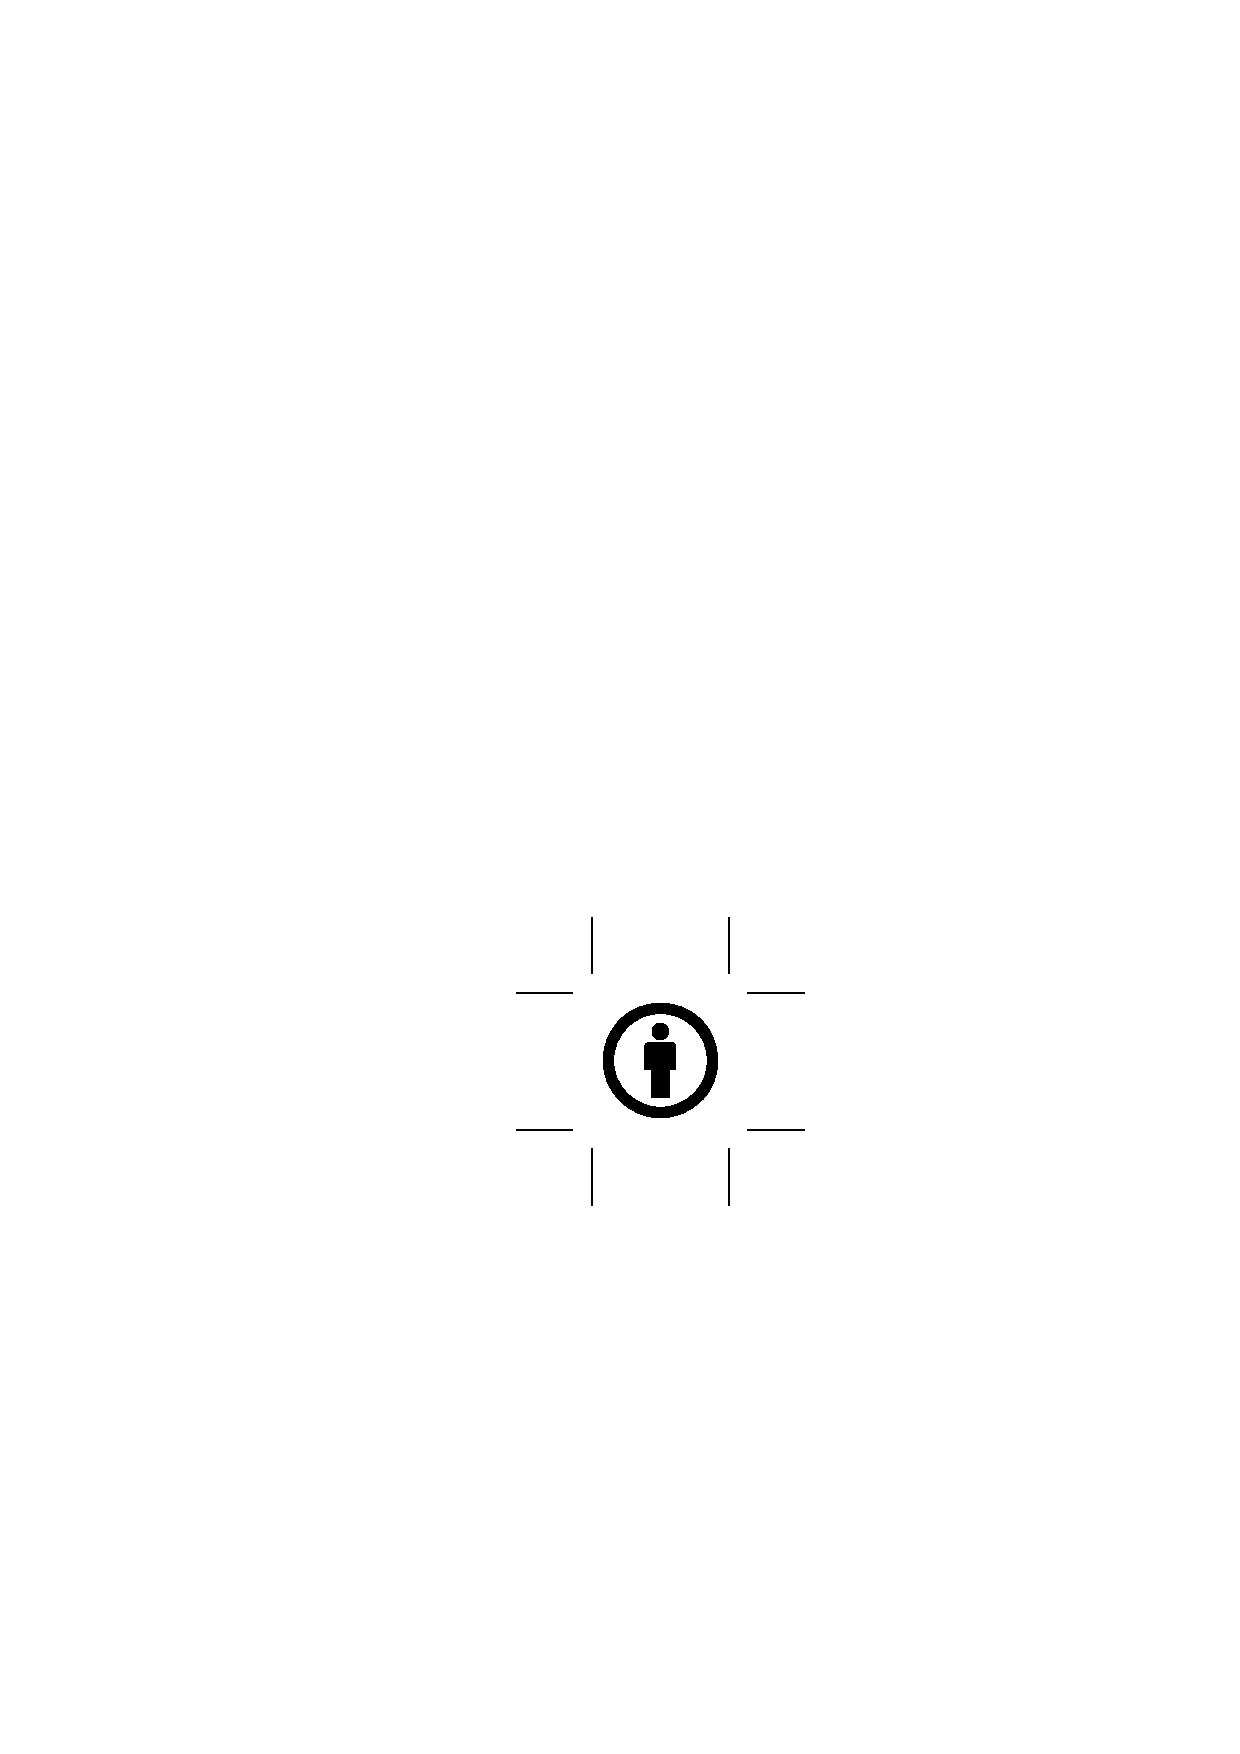
\includegraphics{cc-icons-eps/by}
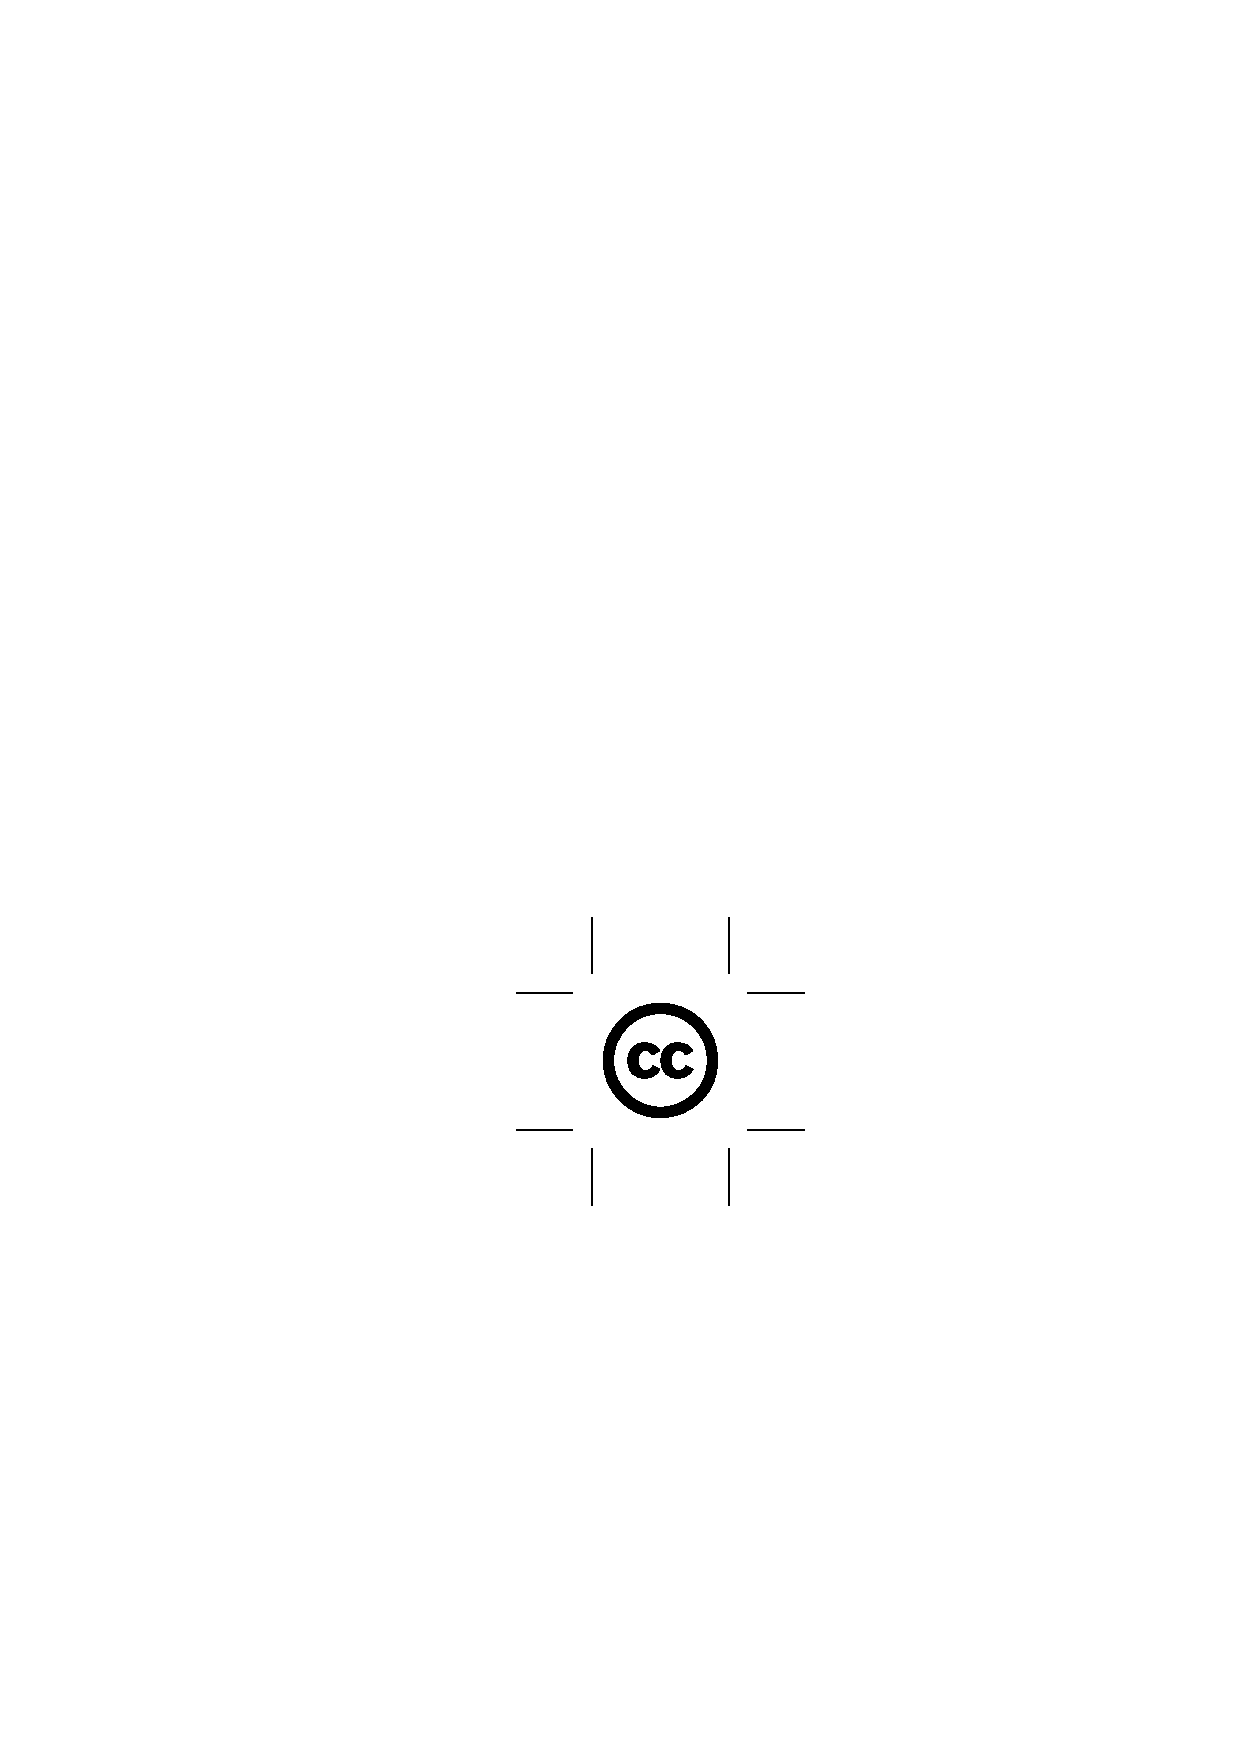
\includegraphics{cc-icons-eps/cc}
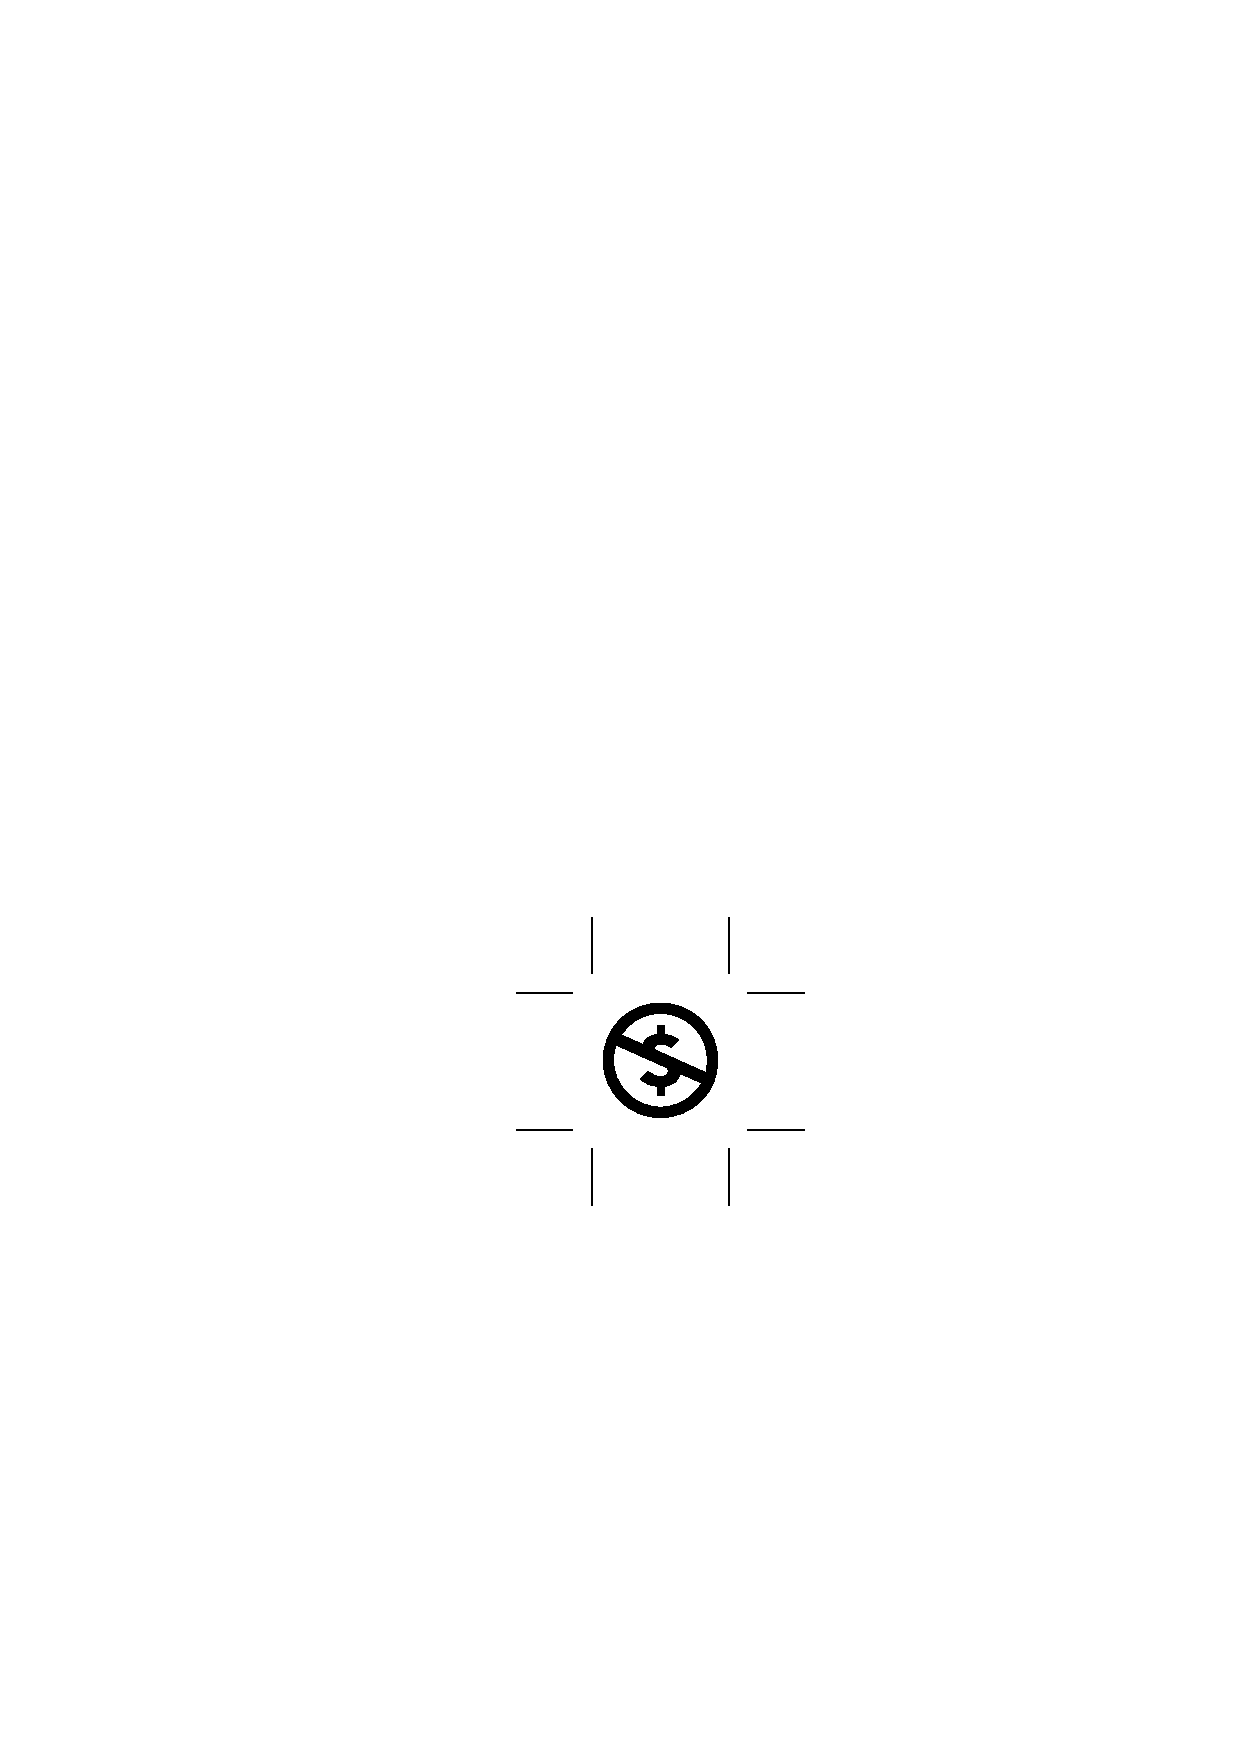
\includegraphics{cc-icons-eps/nc}
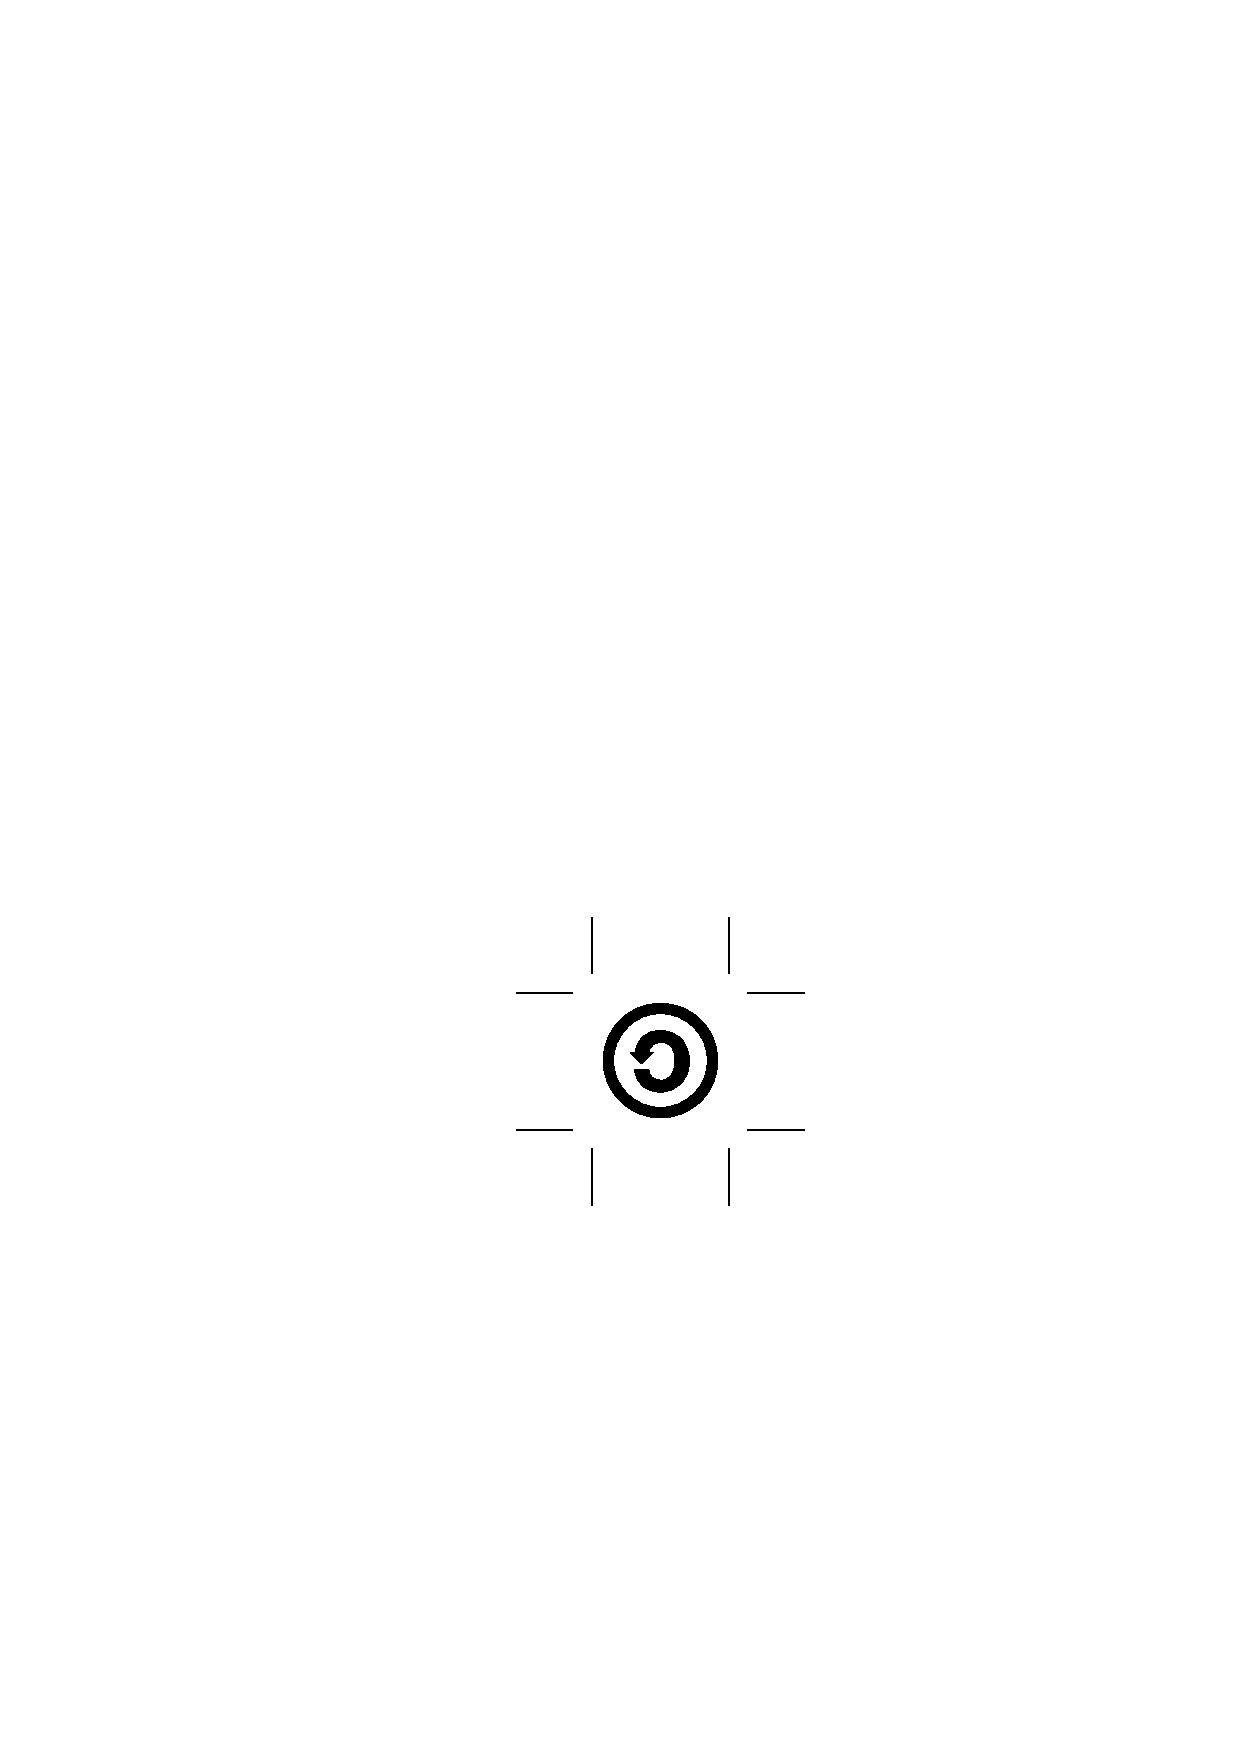
\includegraphics{cc-icons-eps/sa}
\end{center}

\subsection*{Octave sources}
All the Java sources are distributed under, where the word ``Software'' is
referred to all of the sources that are present in this work: \\
\textbf{
Copyright (c) 2011 Massimo Nocentini\\
Permission is hereby granted, free of charge, to any person obtaining a copy of
this software and associated documentation files (the "Software"), to deal in 
the Software without restriction, including without limitation the rights to 
use, copy, modify, merge, publish, distribute, sublicense, and/or sell 
copies of the Software, and to permit persons to whom the Software is furnished 
to do so, subject to the following conditions:\\
The above copyright notice and this permission notice shall be included in all 
copies or substantial portions of the Software.\\
THE SOFTWARE IS PROVIDED "AS IS", WITHOUT WARRANTY OF ANY KIND, EXPRESS OR 
IMPLIED, INCLUDING BUT NOT LIMITED TO THE WARRANTIES OF MERCHANTABILITY, 
FITNESS FOR A PARTICULAR PURPOSE AND NONINFRINGEMENT. IN NO EVENT SHALL THE 
AUTHORS OR COPYRIGHT HOLDERS BE LIABLE FOR ANY CLAIM, DAMAGES OR OTHER LIABILITY, 
WHETHER IN AN ACTION OF CONTRACT, TORT OR OTHERWISE, ARISING FROM, OUT OF OR IN 
CONNECTION WITH THE SOFTWARE OR THE USE OR OTHER DEALINGS IN THE SOFTWARE.
}
